\documentclass[oneside, class=book, 12pt, crop=false]{standalone}

\usepackage{../dissertationstyle}

\bibliography{../personal}

\begin{document}

\ifstandalone
  \graphicspath{ {./images/} }
  \setcounter{chapter}{2}
  \chapter{Implementation}
\fi
\resetfigpath{implementation}

In this chapter, we discuss the software that was produced during this project. We begin by discussing the structure of the project at a high-level, and then cover the high-level structure of the source code repository. Then, we briefly discuss the data synthesis component of the project. Finally, we detail and justify the algorithms and implementation for the metric calculators, similarity scorers, and transformations.

\section{Project Structure}

The project consists of two major components: data synthesis and the classifier. The data synthesis module is relatively simple, and was only of use for early testing stages of the project where real-world data was not available. Because of this, we only briefly discuss the data synthesis component.

A diagram outlining the structure of the data synthesis component is given in Figure \ref{fig:datasynthesisflow}. A MusicXML score is passed into the parser, which converts the score into a more useful form for audio generation. This parsed score, along with a pianist profile fed with some parameters, are passed into an audio generation component, which applies slight modifications to the score based on the pianist profile, and finally synthesises the audio as a WAV file.

\begin{figure}[h]
  \centering
  \begin{tikzpicture}[
  squarednode/.style={rectangle, draw=black!100, fill=black!10, very thick, minimum size=6.5mm},
  datanode/.style={rectangle, draw=black!100, fill=black!0, very thick, minimum size=6.5mm},
  ]
  %Nodes
  \node[datanode] (mxl) {MusicXML Score};
  \node[squarednode] (mxlparser) [right= of mxl] {MusicXML Parser};
  \node[squarednode] (profile) [below= 2.5cm of mxlparser] {Pianist Profile};
  \node[datanode] (tempoenvelope) [below left=of profile] {Tempo Envelope};
  \node[datanode] (amplitudedist) [below= 2 of profile] {Amplitude Distribution};
  \node[datanode] (accuracy) [below right=  of profile] {Timing Accuracy};
  \node[squarednode] (audiogenerator) [below right=of mxlparser] {Audio Generator};
  \node[datanode] (audio) [right= of audiogenerator] {Audio};

  \draw[->] (mxl.east) -- (mxlparser.west);
  \draw[->] (tempoenvelope.east) -| ([xshift=-5pt]profile.south);
  \draw[->] (amplitudedist.north) -- (profile.south);
  \draw[->] (accuracy.west) -| ([xshift=5pt]profile.south);
  \draw[->] (mxlparser.south) |- ([yshift=3pt]audiogenerator.west);
  \draw[->] (profile.north) |- ([yshift=-3pt]audiogenerator.west);
  \draw[->] (audiogenerator.east) -- (audio.west);
  \end{tikzpicture}
  \caption{Flowchart of the data synthesis component}
  \label{fig:datasynthesisflow}
    
\end{figure}


A diagram outlining the structure of the classifier is given in Figure \ref{fig:classifierflow}. Known recordings are passed into the metric calculators, and their metrics stored. To find the performer of an unknown recording, we calculate its metrics, and compare these to the metrics of the known performances using the similarity scorer. We take the most similar performance, and that gives us our performer.

\begin{figure}[h]
  \centering
  \begin{tikzpicture}[
  squarednode/.style={rectangle, draw=black!100, fill=black!10, very thick, minimum size=6.5mm},
  datanode/.style={rectangle, draw=black!100, fill=black!0, very thick, minimum size=6.5mm},
  ]
  %Nodes
  \foreach \x in {2.0, 2.1, 2.2}\node[datanode] at (\x, \x) (knownrecordings) {Known recordings};
  \node[squarednode]      (metriccalculators1)       [right= of knownrecordings] {Metric calculators};
  \node[database, label=left:Stored Metrics, database radius=0.75cm, database segment height=0.375cm]         (storedmetrics)            [below=of metriccalculators1] {};
  \node[squarednode]      (metriccalculators2) [below= 2.5cm of storedmetrics] {Metric calculators};
  \node[datanode]      (unknownrecording)  [left= of metriccalculators2] {Unknown recording};
  \node[squarednode]      (similaritycalculator) [below right= 1cm and 2cm of storedmetrics] {Similarity scorer};
  \node[datanode]       (performer) [right= of similaritycalculator] {Performer};

  %Lines
  \draw[->] (knownrecordings.east) -- (metriccalculators1.west);
  \draw[->] (metriccalculators1.south) -- (storedmetrics.north);
  \draw[->] (unknownrecording.east)  -- (metriccalculators2.west);
  \draw[->] (storedmetrics.south) |- ([yshift=3pt]similaritycalculator.west);
  \draw[->] (metriccalculators2.north) |- ([yshift=-3pt]similaritycalculator.west);
  \draw[->] (similaritycalculator.east) -- (performer.west);

  \end{tikzpicture}

\caption{Flowchart of the core of the classifier}
\label{fig:classifierflow}
\end{figure}

\section{Repository Overview}

A high-level overview of the repository is given in Figure \ref{fig:repositoryoverview}. A high-level distinction is made between source code in the \texttt{src/} directory and data/resources in the \texttt{res/} directory. Within each of these directories, files are further grouped by their purpose and what component of the overall system they belong to.

\begin{figure}[h]
\begin{verbatim}
|-- res/
|   |-- data/
|   |   contains all of the piano recordings
|   |-- irs/
|   |   contains samples of impulse responses for reverb
|   |-- noise/
|   |   contains samples of background noise
|   |-- scores/
|   |   contains MusicXML scores
|   `-- soundfonts/
|       contains soundfonts for data synthesis
`-- src/
    |-- classifier/
    |   |   contains a variety of utility files
    |   |-- metrics/
    |   |   contains metric calculators and similarity scorers
    |   `-- transformations/
    |       contains transformation implementations
    `-- data_synthesis/
        contains all of the data synthesis implementation
\end{verbatim}
\caption{Repository overview}
\label{fig:repositoryoverview}
\end{figure}

All of the code was written by the dissertation author. All files in the \texttt{res/data/} directory were created by the dissertation author, and all other files in the \texttt{res/} directory were found online.

Files in the \texttt{irs/} directory were taken from the University of York's \href{https://www.openairlib.net}{OpenAir} project under the Creative Commons 4.0 License\footnote{\url{https://creativecommons.org/licenses/by/4.0/}}.

All other files were taken using the Creative Commons 1.0 license.

\section{Data Synthesis}\label{sec:datasynthesis}

In this section we discuss the implementation of the data synthesis module created for generating data to test the metric calculators on during development. This involved a MusicXML parser, pianist profiles, and synthesising audio.

\subsection{MusicXML Parser}

MusicXML is a file format designed to score music scores for computer-readability \cite{musicxml}. It specifies a number of XML tags and their usage relating to musical structure.

The parser simply needs to understand each of these tags, and convert the XML into a format that is usable for audio generation. The format we want to turn the MusicXML into is essentially a list of \texttt{Note} objects (defined in \texttt{src/data\_synthesis/piece.py}), where each \texttt{Note} specifies a pitch, start time, and duration. From this, we can easily generate audio.

The parser is simple and linear, we never need to do any backtracking. We consume each tag in turn, keeping track of book-keeping information when necessary. This book-keeping information is mostly in the form of `voices' and `ties'.

The \texttt{<note>} tag does not specify a start time, it is instead implied by the durations of all previous notes. This means that in order to have multiple notes play at the same time, we need the concept of voices. Each voice progresses in time independently, and each \texttt{<note>} specifies a voice, so we simply keep track of all of the voices progress to find the start and end time for each note.

In music, tied notes are notes of the same pitch that occur adjacently, along with a tie marking. Tied notes are played instead as a single note, with subsequent tied notes indicating extra duration. In MusicXML, tied notes generate multiple \texttt{<note>} tags, so we should not always generate a new note to play when we see a \texttt{<note>} tag. We have to keep track of whether or not the previous note was tied, and if it was then we simply extend the duration of the previous note.
% TODO: include picture of tied note?

\subsection{Pianist Profiles}

Pianist profiles are a construct to introduce artificial variation into the \texttt{Piece}s generated by the MusicXML parser, in order to verify that the metric calculators are producing sensible results.

A pianist profile allows for three ways to introduce variation: a tempo envelope, which specifies changes in tempo over the whole piece; an amplitude distribution, which specifies a probability distribution to sample note volumes from; and an offset distribution, specifies a probability distribution to sample note offsets (from their expected start times) from.

A \texttt{Profile} object can then be applied to a \texttt{Piece} object to generate a new \texttt{Piece} with the added variation.

\subsection{Audio Synthesis}

To synthesise audio, we make use of the \texttt{fluidsynth} library for Python. Using this library means that all we have to do is supply a soundfont and a number of note-on and note-off events and we can generate an audio file.

A soundfont is effectively a collection of samples, that specifies how to generate audio for a note with a given pitch and duration.

Then, as designed, our \texttt{Piece} class makes it very easily to generate note-on and note-off events. For each note in our piece, we can generate a corresponding note-on and note-off event from its start time and duration. Once generating these events for all notes, we can simply sort them by time and handle them one-by-one, and \texttt{fluidsynth} will generate an audio signal for us.


\section{Metric Calculators}

In this section we detail and justify the specific algorithms used for each of the metric calculators.

The structure of this implementation is designed around modularity: it should be easy to create new metric calculators and have them evaluated. For this, we want each metric calculator to implement a function that calculates a metric given some audio, and a function that calculates the similarity between two metrics. To do this, we define a class \texttt{MetricCalculator} in \texttt{src/classifier/metrics/metric.py} with three functions: \texttt{\_\_init\_\_()} (a constructor), \texttt{calculate\_metric(audio)}, and \texttt{calculate\_similarity(audio1, audio2, metric1, metric2)}. Python3 does not support abstract/virtual methods, so we instead define each of these functions to raise a \texttt{NotImplementedError} on call, forcing all classes that inherit from it to override these methods.


\begin{itemize}
  \item
The \texttt{\_\_init\_\_()} method allows the user to pass parameters to a metric calculator (like window advance/size), such that each call to the calculations uses the same parameters.

\item
  The \texttt{calculate\_metric(audio)} method takes as a parameter an \texttt{Audio} object (which essentially holds a signal, some extra metadata like sample rate and name, and caches metrics for faster evaluation times), which should be all it needs to calculate a metric.

\item
  The \texttt{calculate\_similarity(audio1, audio2, metric1, metric2)} method takes as parameter two \texttt{Audio} objects and two metrics, the form of which is defined by the return value of the \texttt{calculate\_metric(audio)} method.

  The reason we need the \texttt{audio1} and \texttt{audio2} parameters is because the audio objects can be used to calculate important information, like the beat timings, so that we can meaningfully compare different metrics.
\end{itemize}

To create a new metric calculator, we just define a class that inherits from \texttt{MetricCalculator} and override the functions with appropriate method definitions.

\subsection{Tempo Variation Over Time}\label{sec:tempovariation}

This metric calculator is implemented in the \texttt{src/classifier/metrics/tempo.py} file.

The computation of this metric builds closely on top of the beat tracking algorithm described in Section \ref{sec:beattracking}. As described before, this beat tracking algorithm works at a high-level by finding points where  many frequencies change in power at one time. For example, in Figure \ref{fig:spectrogrambeats}, we clearly see note onsets in the spectrogram since the power of the frequency bands drastically changes.

\begin{figure}[h]
  \centering
  \captionsetup{justification=centering}
  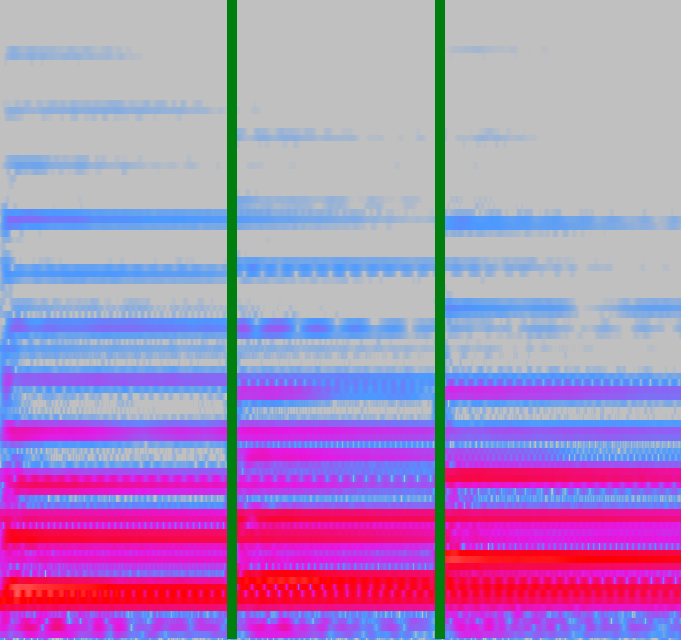
\includegraphics[scale=0.3]{spectrogram}
  \caption{Spectrogram of an excerpt of a piano performance. Note onsets are manually marked in green}
  \label{fig:spectrogrambeats}
\end{figure}

In fact, all we do is run our beat tracking algorithm on our audio and take the first-order difference between our beat times, and then apply smoothing by taking the moving average to reduce the impact of micro-variations in note timings (which we instead capture with the note offsets metric). 

There were a few other choices for constructing this metric, for example instead of taking the first-order difference of our beat times, we could simply use the beat times themselves. To see the issues with this approach, suppose we have two performances that have very similar tempos in the latter half, but are different in the first half. We would like to consider these performances reasonably similar since the tempos are similar in the latter half, but by taking the absolute beat times we are unable to find any similarity since the differing tempos in the first half will offset the beat times in the latter half. Taking the first-order difference avoids this issue. Another option might be taking higher-order differences, which seems like it might have some merits. For example, a second-order difference would allow us to easily find where a piece is speeding up/slowing down as opposed to just fast/slow, but by doing this we lose the information on whether the piece actually is being played fast/slow, which isn't ideal.

Furthermore, the smoothing we perform is very important. Being able to avoid these micro-variations is incredibly useful, since this metric really intends to capture an overall view of how tempo changes over the performance of the piece, and not a microscopic view of timings within each bar, for example.

We are also able to tune how much of this smoothing we get on our beat time differences by changing the window size of our moving average. For our case, we choose a window size of 4 beats, which corresponds to the length of a bar (the next level up in the temporal structure of music) in most Western European music, which is what our dataset consists of.

Our tempo variation over time metric is then calculated as follows, which includes operation of the beat tracking algorithm described in Section \ref{sec:beattracking}.

\begin{enumerate}[label=\textbf{Step \arabic*:}]
  \item
    Calculate the onset function of our audio signal.

  \item
    Take the correlation between delayed versions of the onset function and itself to find an estimate for the overall tempo of the performance.
    
  \item
    Use Ellis' dynamics programming algorithm to calculate the beat times in our performance.

  \item
    Take the first-order difference of these beat times and take a moving average as our final metric.
    Take the first-order difference of these beat times and take a moving average as our final metric.

    
\end{enumerate}

\subsubsection{Similarity Scorer}\label{sec:temposimilarity}

To calculate the similarity between two tempo metrics we use a technique which we will frequently see in the similarity scorers for other metrics: calculating the mean squared error. We can consider our tempo metric as being a function of beat number, returning us the time difference between the last beat. Then, to calculate the similarity between two metrics, we just take the mean squared error between these two functions (truncating the longer function if necessary), giving us a number we call $\varepsilon$.

This is not yet useful as a similarity score, however, since it can grow unboundedly large, so we return the error as $e^{-\varepsilon}$. The intuition behind the choice of this transformation is that if our two performances are the same, we expect $\varepsilon$ to be equal to 0, and thus $e^{-\varepsilon}$ will be 1. As $\varepsilon$ grows, $e^{-\varepsilon}$ will approach 0, which gives us a useful similarity score.

\subsection{Dynamics Over Time}

This metric calculator is implemented in the \texttt{src/classifier/metrics/dynamics.py} file.

For this metric, we want to infer an envelope of our signal that represents the loudness over time. Since the amplitude of a signal at any point represents its loudness, a good metric should follow a similar shape to the waveform of the signal, like as seen earlier in Figure \ref{figure:dynamicsplot}

Given that, as we have seen the amplitude of the signal roughly corresponds to its loudness, it might seem sensible to just use the waveform itself as our dynamics metric, but this has a few problems:

\begin{enumerate}[label=\textbf{Problem \arabic*:}]
  \item
    Sound signals contain oscillating values (between positive and negative), and it does not make sense for the dynamics of our signal to quickly oscillate between high values and low values.

  \item
    We have too much granularity, which means that noise in our signal might cause more significant performance drops.

  \item
    There is a huge range of magnitudes in the amplitudes of our signal

  \item
    Humans perceive different frequencies at different volumes, even for the same intensity.
\end{enumerate}

To solve problem 1, we can simply perform some operation like taking the absolute value, or squaring, to ensure the value is always positive. To solve problem 2, we can take a sliding window over our signal and compute our loudness value over this signal excerpt, as opposed to a single point. To solve problem 3, we can take the log of our loudness value. Finally, to solve problem 4, we can apply some weightings to different frequencies.

All of this leads to the following algorithm for computing our dynamics metric:

\begin{enumerate}[label=\textbf{Step \arabic*:}]
  \item
    First, take windows of the signal. We use a window size of 0.16 seconds and a window advance of 0.04 seconds. This solves problem 2.

  \item
    For each window, calculate its power spectrum (by computing its Fourier transform and calculating the energy in each frequency band). This solves problem 1 (the power spectrum is always positive), and will help us solve problem 4 later.

  \item
    Convert the power spectrum to use the mel scale, so that the frequency bands are perceptually distributed.

  \item
    Convert the mel power spectrum into decibels, which is essentially using a log scale, solving problem 3.

  \item
    Weight each of the decibel values by the frequency band that it is in. We use the ITU-R 468 weighting \cite{itu86}. This solves problem 4.

  \item
    Compute the aggregate adjusted noise level by converting the weighted decibel values to a linear scale, summing them, and converting back to decibels.
\end{enumerate}

There are a few important considerations with this algorithm. When converting to decibels, like in step 4, we need a reference value, since decibels is inherently a relative scale. We could, for example, choose the reference point to be the maximum power in the signal (meaning the decibel values are normalised to have a peak of 0dB), but this means that we would no longer be able to compare absolute volume differences between performances, only the shape of the dynamics over time. So, it is important that we choose a fixed reference point, although the actual value of the reference point does not matter too much.

Furthermore, the choice of frequency weighting also requires consideration. We choose the standard used by the International Telecommunication Union, which can be seen in Figure \ref{fig:itu468}. We make this choice over other curves, like the A-weighting curve \cite{bisch05}, since these curves often have other issues like only being valid for pure sine waves, which our data is definitely not. The use of the ITU-R 468 curve across the world also gives us confidence that this curve is sensible.

\begin{figure}[h]
  \centering
  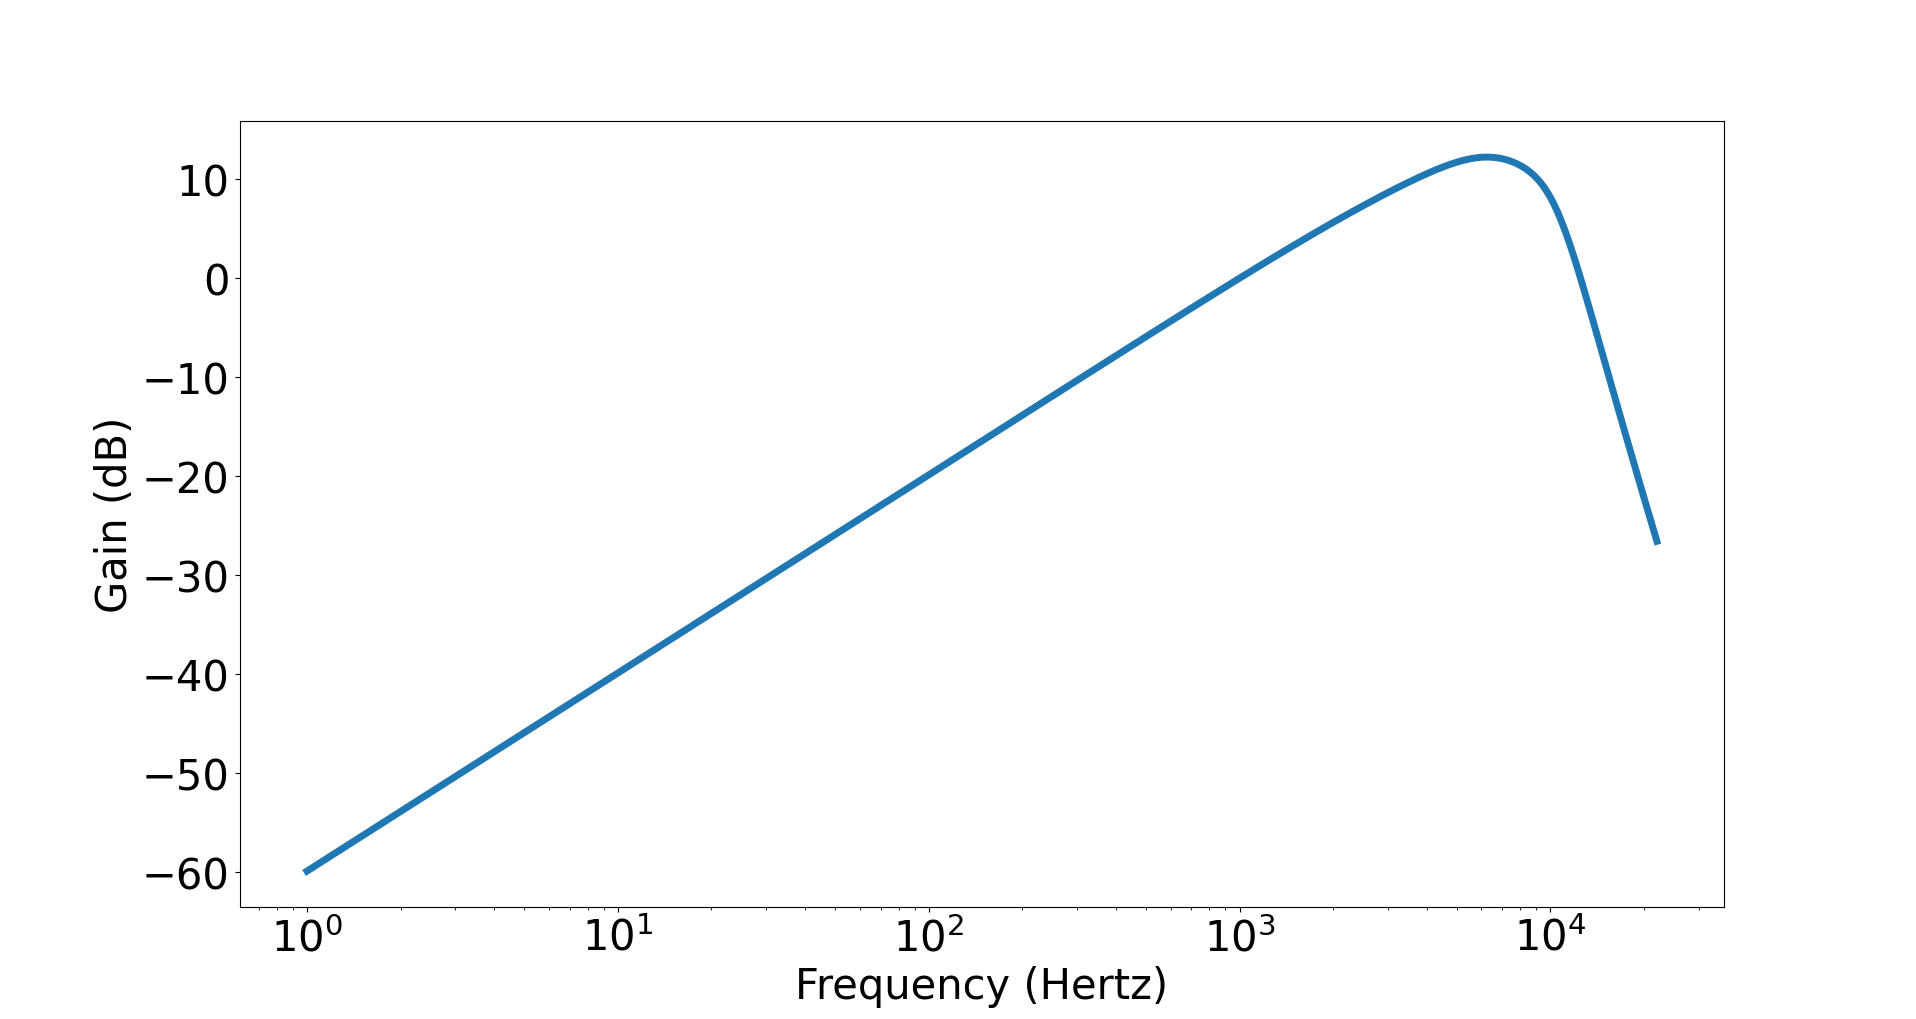
\includegraphics[scale=0.3]{itu468} 
  \caption{The ITU-R 468 frequency weighting curve}
  \label{fig:itu468}
\end{figure}

\subsubsection{Similarity Scorer}

The similarity scorer for the dynamics metric uses similar techniques as the other metrics, which are described in Section \ref{sec:temposimilarity}.

As before, we begin by truncating the longer metric if necessary. Then, we perform a step of normalisation: we only care about relative difference between the two metrics, so we normalise both arrays such that the value of 1 represents the highest value found in both metrics.

Finally, as before, we calculate the mean squared error between these normalised arrays, and apply the negative exponential function to generate our similarity score.


\subsection{Chroma Vector Extraction}

This metric is implemented in the \texttt{src/classifier/metrics/chroma.py} file.

This metric tries to capture the notes that are being played at a particular time in the performance, which is useful if a performer consistently plays wrong notes at certain points, or uses the sustain pedal in a particular way (which extends the duration of notes, which can create the illusion that many notes are being played simultaneously).

Since this system is designed just for use with piano, we can therefore restrict ourselves to the twelve-tone scale found in most Western music, where each octave is split into 12 equally distanced notes. This means that the current implementation of this metric would be unsuitable for music that lies outside of this musical system, like micro-tonal music.

For this metric, we also decide not to determine which octave the notes lie in, and instead consider the 12 tones irrespective of their octave. This is because it can be difficult to distinguish the same note in different octaves, since the frequency content is so similar. % (as seen in Figure blahblah).

So, we can now define a chroma vector as being a 12-element vector, where each element corresponds to the `strength' of a particular note, as seen earlier in Figure \ref{figure:chromaplot}. Our metric is then just an array of these chroma vectors over time.

To calculate a chroma vector, we look at the frequency content of our signal, and for each possible note (here, we make a distinction between notes in different octaves), summing up the frequency content for that note's frequency band, and adding it to the corresponding element of our chroma vector.

\begin{enumerate}[label=\textbf{Step \arabic*:}]
  \item
    First, take windows of our signal. We use a window size of 0.1 seconds and a window advance of 0.025 seconds.

  \item
    For each window, calculate its chroma vector:

    \begin{enumerate}
      \item
        Initialise our chroma vector to all zeros.

      \item

        Calculate the spectrum of the signal using the real Fourier transform.

      \item
        Iterate over each possible note, and calculate its frequency band by finding the lower and upper frequency bounds at half a note lower and higher than the note respectively.

        For `possible note' here, we mean any note within the range of the lowest and highest notes on a piano, which are at around 27.5 Hz  and 4186.0 Hz respectively.

      \item
        Sum the values in the spectrum within that frequency band, and add that value to the corresponding chroma vector element.
    \end{enumerate}
\end{enumerate}


\subsubsection{Similarity Scorer}\label{sec:chroma similarity}


We again apply similar techniques as used in other similarity scorers: truncating to the shorter metric length, calculating the mean squared error between the two metrics, and applying the negative exponential function.

There is one major difference between this similarity scorer and others, however. For the chroma similarity, we only compare the metric at the detected beat times. This has some benefits over the naive method of just taking the mean squared error over the entire metric. If we use the naive method, then when we compare the metrics, we may be comparing different parts of the piece entirely since the tempos of the two performances are likely to differ. By ensuring that we only compare the metrics at each beat time, we can be certain that we are comparing the metrics meaningfully.

There are some downsides to this approach. For example, if a note is held for a long time in one performance, but is held only for a short time in another performance, then this similarity scorer will be unable to detect this, since it only compares the metrics at instantaneous beat times. However, we might hope that our dynamics metric might be able to capture this behaviour instead, so combining these two metrics should be able to overcome this shortcoming.



\subsection{Note Offsets}

This metric is implemented in the \texttt{src/classifier/metrics/offsets.py} file.

This metric tries to capture micro-variations in rhythm from a performer, in some sense how `accurate' their playing of notes is. Unlike the other metrics that generate some kind of function/curve from the audio signal, this metric instead works by modelling the performer's micro-variations as a probability distribution, and we just return the parameters of this probability distribution.

We do this because it is unlikely a performer would reliably have the same micro-variations at each note that is played. This means that if we were to, for example, store for each beat the time difference (offset) between the beat and when the performer actually played the note, and then for our similarity scorer calculated the mean squared error between each beat's offset, we would be unlikely to obtain good results (Note for John: I have data that supports this, getting around a 14\% success rate with this proposed naive solution, compared to around 65\% with the current technique. Is that worth mentioning here, or should I wait until the evaluation section?).

So, from the offsets we generate the mean and standard deviation for a normal distribution, representing when they are most likely to play a note relative to the expected beat time. Figure \ref{fig:offsetdists} shows plots of inferred probability distributions for different performers and the same performer, respectively. Our algorithm works as follows:

\begin{enumerate}[label=\textbf{Step \arabic*:}]
  \item
    Take a moving average of the first-order difference of the beat times to obtain a smoothed tempo curve, in the same way we calculate the tempo metric in Section \ref{sec:tempovariation}.

  \item
    For each beat time in the cumulative sum of the smoothed tempo curve, find the nearest onset and record its displacement from the expected beat time.

    We do this by searching a small window (0.1 seconds) around our expected beat time in our onset function (defined in Section \ref{subsec:onset detection}), and choosing the value with the highest onset.

  \item
    Calculate and return the mean and standard deviation of the displacements.

    
\end{enumerate}

\begin{figure}[h]
  \captionsetup{justification=centering}
  \centering
  \begin{subfigure}[b]{\textwidth}
    \centering
    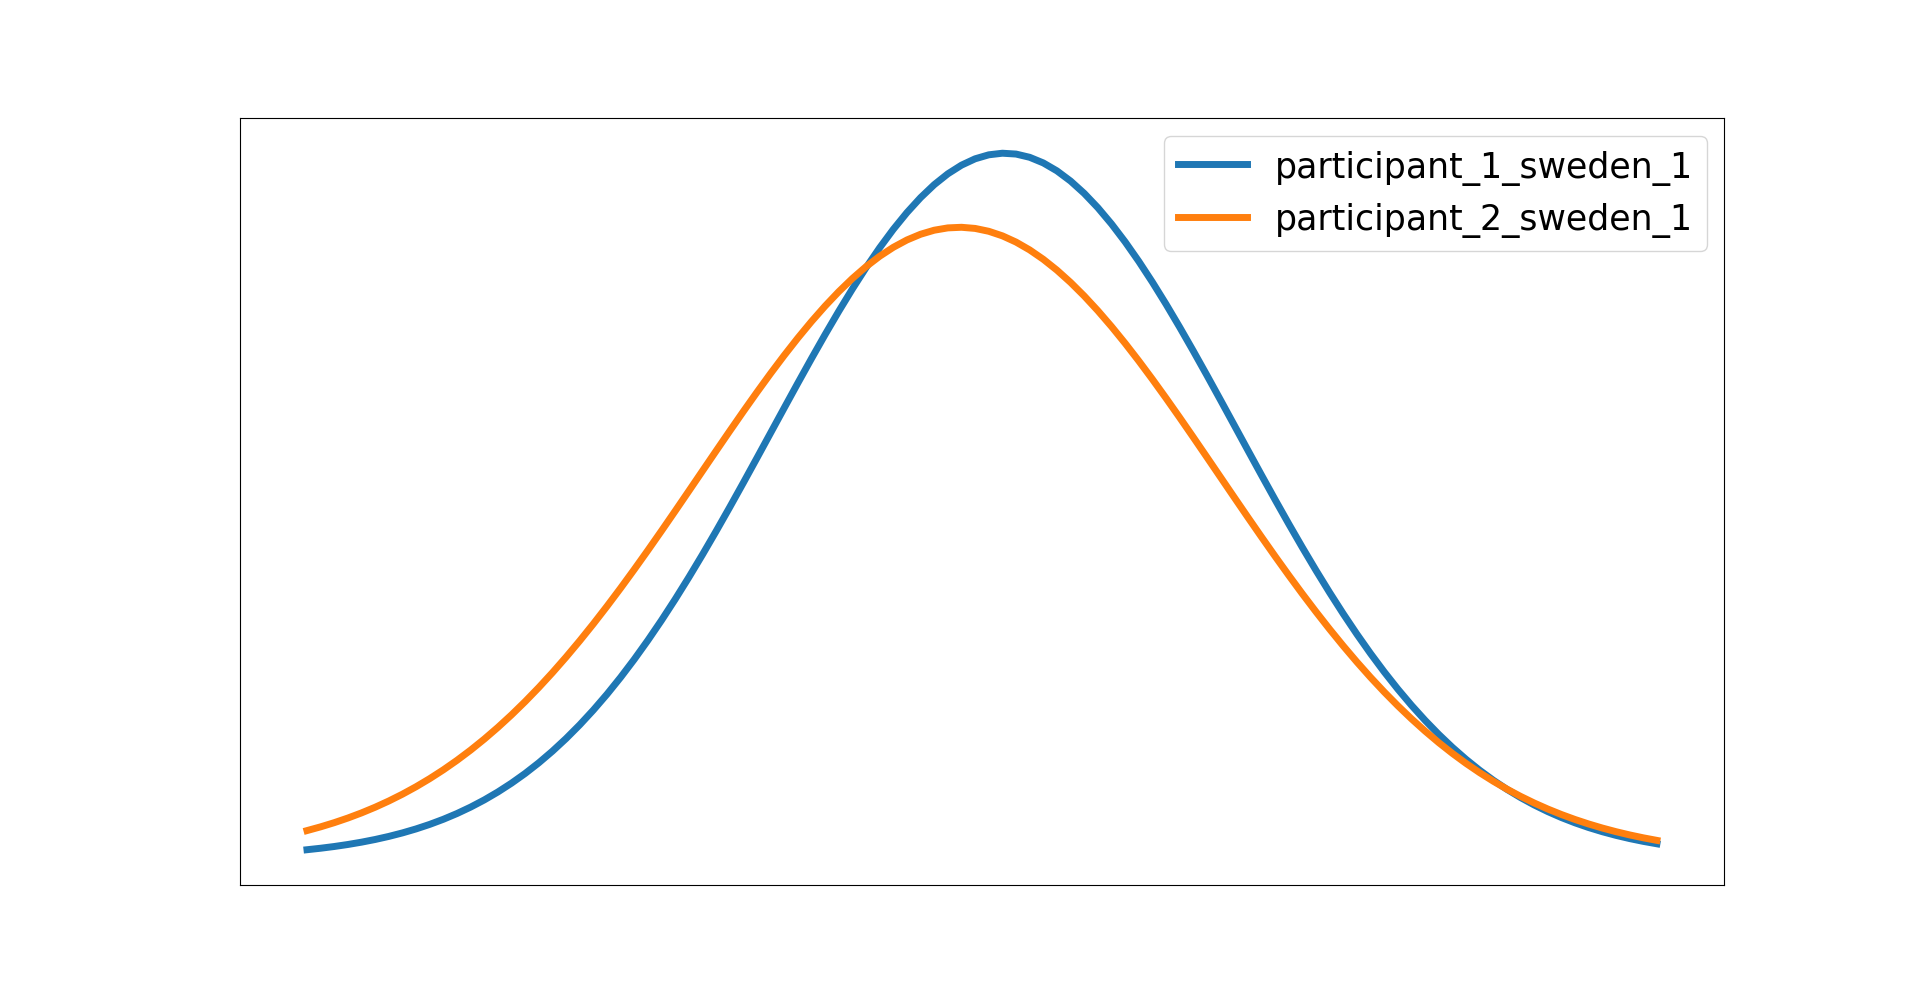
\includegraphics[scale=0.25]{offsetdist1}
    \label{fig:offsetdist1}
    \caption{}
  \end{subfigure}

  \begin{subfigure}[b]{\textwidth}
    \centering
    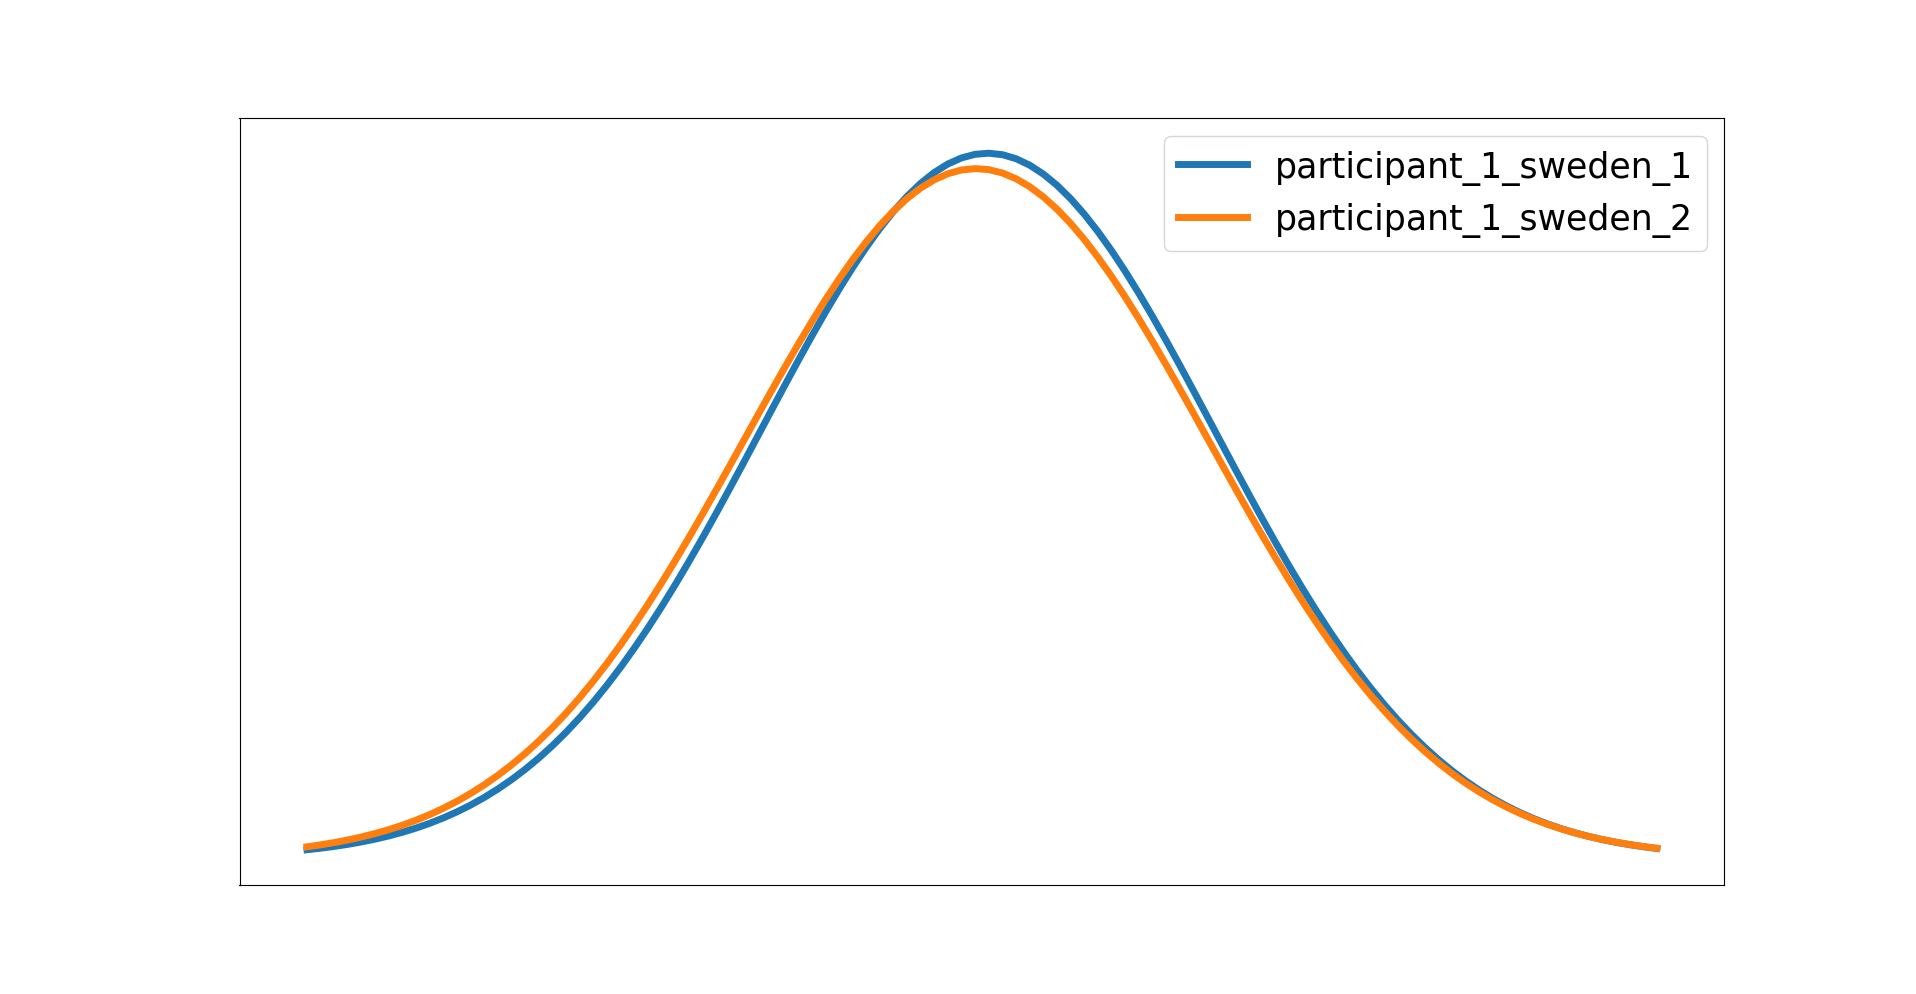
\includegraphics[scale=0.25]{offsetdist2}
    \caption{}
  \end{subfigure}
  \caption{Inferred probability distributions for different performers (a) and the same performer (b)}
  \label{fig:offsetdists}
\end{figure}

\subsubsection{Similarity Scorer}

In essence, the similarity scorer for this metric is about comparing two probability distributions. For this reason, we use an information theoretic approach for the similarity scorer. In particular, we use the Kullback-Leibler divergence $D_{KL}(P||Q)$ that calculates a `distance' between two probability distributions $P$ and $Q$.

We do not just return $D_{KL}(P||Q)$ as our similarity however, since it is by definition asymmetric, and it is important that our similarity scorers are symmetric. Furthermore, $D_{KL}(P||Q)$ generally treats $P$ as some kind of `true' distribution. So, we instead symmetrise this measure and calculate $\frac{D_{KL}(P||Q) + D_{KL}(Q||P)}{2}$ instead.

\begin{equation}\label{eq:dkl}
  D_{KL}(P||Q) = \int_{-\infty}^\infty p(x) \log \frac{p(x)}{q(x)} \mathrm{d}x
\end{equation}

The calculation of this metric is relatively easy. The definition of $D_{KL}(P||Q)$ is given in Equation \ref{eq:dkl}, and since our metric specifies a normal distribution, if our metrics are modelled $M_1 \sim N(\mu_1, \sigma_1^2)$ and $M_2 \sim N(\mu_2, \sigma_2^2)$, then we can derive an expression for $D_{KL}(M_1||M_2)$ seen in Equation \ref{eq:dkl2}

\begin{equation}\label{eq:dkl2}
  D_{KL}(M_1||M_2) = \log \frac{\sigma_2}{\sigma_1} + \frac{\sigma_1^2 + (\mu_1 - \mu_2)^2}{2\sigma_2^2} - \frac{1}{2}
\end{equation}

From this, we can derive an expression for $\frac{D_{KL}(M_1 || M_2) - D_{KL}(M_2 || M_1)}{2}$, given in Equation \ref{eq:dkl3}

\begin{equation}\label{eq:dkl3}
  \frac{D_{KL}(M_1 || M_2) - D_{KL}(M_2||M_1)}{2} = \frac{\sigma_1^4 + \sigma_2^4 + (\sigma_1^2 + \sigma_2^2)(\mu_1 - \mu_2)^2}{4\sigma_1^2\sigma_2^2} - \frac{1}{2}
\end{equation}

We can see that if $\sigma_1 = \sigma_2$ and $\mu_1 = \mu_2$, that this symmetrised divergence becomes 0, and as as the parameters begin to differ, the divergence will get larger. This means that we can calculate our final similarity score as the negative exponential of our symmetrised divergence, which will be 1 when the distributions are the same, and approach 0 as the distributions differ.

\subsection{Timbre extraction}\label{sec:timbre metric}

The timbre of a sound can be thought of as the `character' of that sound. For example, if a trumpet and harp both play the same note they will sound different, because the timbres of these notes are different. So, this metric aims to find and quantify timbral differences between performers. It is to be expected that this is difficult, since quantifying timbre is known to be a difficult problem.

The timbre of a sound comes from its harmonic content, i.e. what frequencies are present above the frequency of the note that is being played. We can see that this differs between instruments by looking at the spectrogram of the same note played on both a saxophone and piano, as seen in Figure \ref{fig:saxpianoc}.

\begin{figure}[h]
  \centering
  \begin{subfigure}[b]{\textwidth}
    \centering
    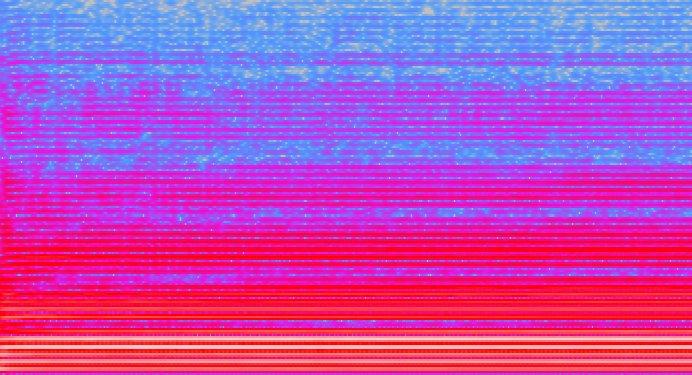
\includegraphics[scale=0.35]{saxc}
    \caption{}
  \end{subfigure}
  \begin{subfigure}[b]{\textwidth}
    \centering
    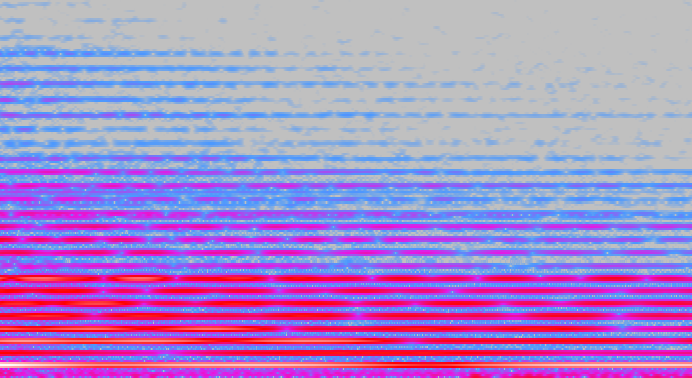
\includegraphics[scale=0.35]{pianoc}
    \caption{}
  \end{subfigure}
  \caption{Spectrogram of the note C played on a saxophone (a) and piano (b)}
  \label{fig:saxpianoc}
\end{figure}

So, our timbre metric needs to capture the harmonic content of an audio signal. It is not just enough to quantify the spectrogram however, since if we did we would be capturing melodic content of the audio signal, i.e. which note is being played, which we want to leave for the chroma metric to capture instead. This means that we would need to normalise the spectrum such that the actual note being played does not matter.

We also only care about the timbre when a note is being played. For this reason, we only calculate our timbre metric at expected beat times. It should be noted that a note will not always occur on an expected beat, but we can assume that a note will occur on most expected beats.

To quantify the spectrum of a signal, we use a standard technique of generating mel-frequency cepstrum coefficients (MFCCs), which is often used for applications like speech recognition and music genre classification. A cepstrum is obtained by first taking the log of the magnitudes in a spectrum, and then taking its inverse Fourier transform. A mel-frequency cepstrum works simply by instead using a power spectrum (like a frequency spectrum, but we square the magnitudes), and then converting the spectrum to use the mel scale first. The MFCCs are then just the magnitudes of the inverse Fourier transformed signal.

Our metric calculator works as follows:

\begin{enumerate}[label=\textbf{Step \arabic*:}]
  \item
    For each beat time, take a window of the signal, we use a window size of 0.3 seconds.

  \item
    Calculate the spectrum of each window by taking its Fourier transform.

  \item
    Find the note that is most likely being played, and shift the spectrum such that this matches a standard note (we use the note A at 440 Hz).

    To find the note that is most likely being played, we use a crude estimation by simply finding the frequency with the largest magnitude. This might fail in the case that multiple notes are being played simultaneously, although in this case no normalisation would be able to remove all of the melodic content.

  \item
    Calculate the MFCCs of the shifted spectrum, using 40 mel bands.
\end{enumerate}

The metric is then an array of the MFCCs for each beat time.

\subsubsection{Similarity Scorer}

The similarity scorer for this metric is simple, and just uses techniques we have seen in previous similarity scorers.

We first truncate each metric to the length of the shorter metric. Then, for each set of MFCCs, we calculate the mean squared error. From this, we can then calculate the mean squared error over the entire metric by finding the mean of these mean squared errors. Finally, we apply the negative exponential function to obtain our similarity score.

\section{Transformations}\label{sec:transformations}

For the purposes of evaluation, we also implement a number of transformations which can be applied to the data before being used in the system. In particular, we implement the addition of background noise as well as the addition of reverb.

A user can specify a number of transformations to apply to evaluation data, as well as the order in which they are applied (since it does not make sense to apply reverb, and then add noise to a signal).

\subsection{Background Noise}

This transformation is implemented in \texttt{src/classifier/transformations/noise.py}.

Background noise is created through a microphone recording additional environmental sounds. The exact set of sources of noise will vary but some sources might include buzzing from electrical equipment, plumbing, speech, etc. This means that synthesising accurate noise is quite difficult. For example, white noise is unlikely to be representative of these sources and thus simply adding Gaussian white noise is unlikely to represent use of the system under data that has real background noise.

Instead of creating a complex system to synthesise background noise, that will inevitably be not completely alike to real background noise, we instead just take samples of background noise and add these samples to our performances.

If we are using samples of background noise, then it is important to consider what happens when the length of our performance exceeds the length of the noise sample. A naive implementation might just repeat the noise sample immediately, but this could lead to artifacts where the amplitude immediately makes a large jump from the end of the signal to the start. One way to avoid these artifacts might be to reverse the noise and then append it to the end, but this might change the character of the noise in some way and make it unrealistic. The solution that we opt for is to have a small period at the end of the noise signal where we overlap another instance of the noise signal. We then cross-fade the two signals, so the volume of the first signal decreases to silence as the volume of the second signal increases from silence. This ensures that we avoid audio artifacts whilst keeping the character of the noise signal.

We also allow for the user to specify the loudness of the noise overall.


\subsection{Reverb}

This transformation is implemented in \texttt{src/classifier/transformations/reverb.py}.

When a sound is played in a room, it will reflect, and be absorbed by, surfaces in the room. These reflections cause an echo-like effect to be heard, and as the sound waves are absorbed, the reverberation becomes diminish until they become inaudible.

%TODO: include diagram of sound with/without reverb

In music production, numerous techniques are used to simulate reverb. There are acoustic techniques like plate or spring reverb which involve passing the sound signal through a metal plate/spring and recording the results, but these acoustic techniques would be infeasible to implement for our application.

A common digital technique is to generate many delayed versions of the signal, as echoes, and play them back. This allows for easy parametrisation and is quick to compute, but is not entirely realistic. The technique we opt for is a more realistic implementation of digital reverb, and uses convolution. We first require a digital recording of the impulse response of a room, which is generated by recording the audio in a room after an impulse, like the popping of a balloon or a clap. Then, we simply convolve this impulse response with our audio signal, which transfers the acoustic characteristics of the room to be transferred onto a performance. This is significantly more computationally expensive than the other digital reverb technique mentioned, but we are not concerned with performance, and instead care much more about the realism of the reverb effect.

\section{Summary}

In this chapter, we have explored the structure of the software implemented, and have justified design decisions made for each of the metric calculators and transformations. This system we have explained was then tested on our gathered dataset, and the results are explored in Chapter \ref{chapter:evaluation}.











% THINGS TO REMEMBER:
% todo: try and change dynamics metric to compare meaningfully between beat times??
%todo: write about no tests
% play two Cs an octave apart for chroma vector extraction section
% show that combination of chroma/dynamics is better, with explanation in chroma similarity scorer
%TODO: also add musical jargon to preparation chapter?












\ifstandalone
  \printbibliography
\fi
    
\end{document}
